\documentclass[12pt, legalpaper]{report}
\usepackage{graphicx}
\graphicspath{{img}}


\title{3DViewer v2.0}
\author{mortylar@student.21-school.ru \\ seftonca@student.21-school.ru \\ audiedet@student.21-school.ru}
\date{\today}

\begin{document}

\maketitle

\chapter{About program}


The program was developed as an educational project for "School 21".
The project implements a program for visualizing a wireframe model in three-dimensional space.
The program was developed in C++ language of the C++17 standard using the GUI library GTK4.

\section{Install}

You can install the program by running the command 
\textbf make install
A folder named "3D\_{}Viewer" will be created in the home directory, which will contain the executable file.

\section{Open}

You can open the program using the command \textbf{make open}

\section{Uninstall}

To remove the program, you can use the command \textbf{make uninstall}

\newpage

\chapter{Main Window}

\section{Main Window}

When you open the program, you will see the main window shown in the picture.
To load the model, you need to click the \textbf{File Button} button and select the model file.
Next, you need to click the \textbf{Load File} button

\begin{figure}[h]
	\centering
	\vspace*{\fill}
	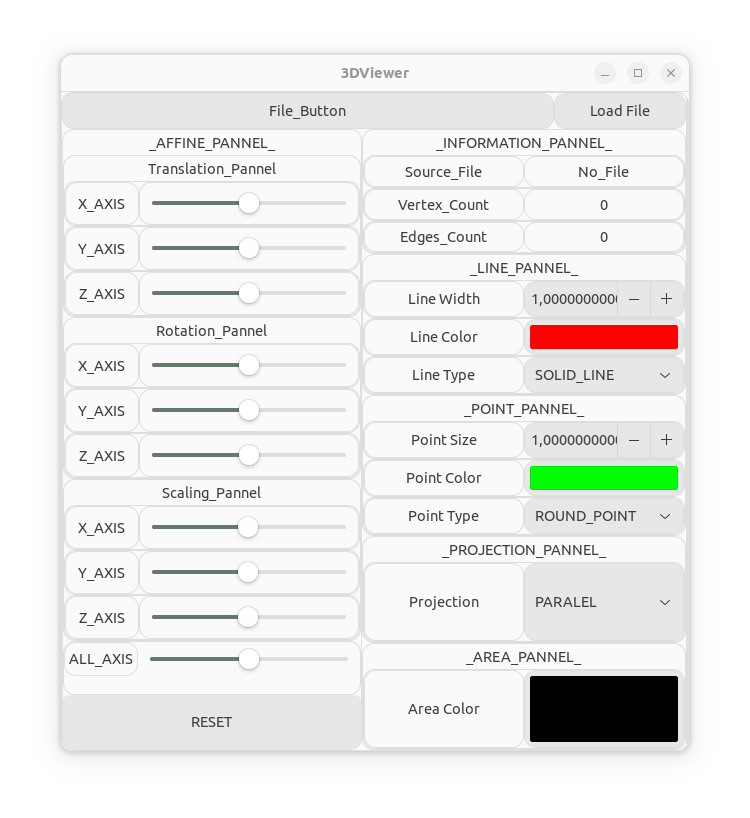
\includegraphics[width=0.5\textwidth]{1}
	\vspace*{\fill}
	\caption{Main Window}
	\label{fig:main}
\end{figure}

\newpage

\chapter{Main functionality}

\begin{itemize}
	\item AFFINE PANNEL consists of:
	\begin{itemize}
		\item \textbf{Translation Panel}.This panel allows you to move the model along three axes X, Y, Z
		\item \textbf{Rotation Panel}.This panel allows you to rotate the model along three axes X, Y, Z
		\item \textbf{Scalling Panel}. This panel allows you to change the scale of the model along three axes X, Y, Z
		\item The \textbf{Reset button} resets all changes to the movement, rotation and scaling of the loaded model.
	\end{itemize}
	\item INFORMATION PANEL. Displays information about the loaded model file, the number of vertices and edges.
	\item LINE PANNEL. Allows you to set the line thickness, select the line color, select the line type: solid line, dotted line, remove lines
	\item POINT PANNEL. Allows you to set the thickness of the dot, select the color of the dot, select the type of dot: triangle, square, circle, do not display dots
	\item PROJECTION PANEL. Allows you to select the projection type: parallel or central
	\item AREA PANNEL. Allows you to set the background color
\end{itemize}

In the right part of the window we see a display of the model in space.

\newpage


\begin{figure}[h]
	\centering
	\vspace*{\fill}
	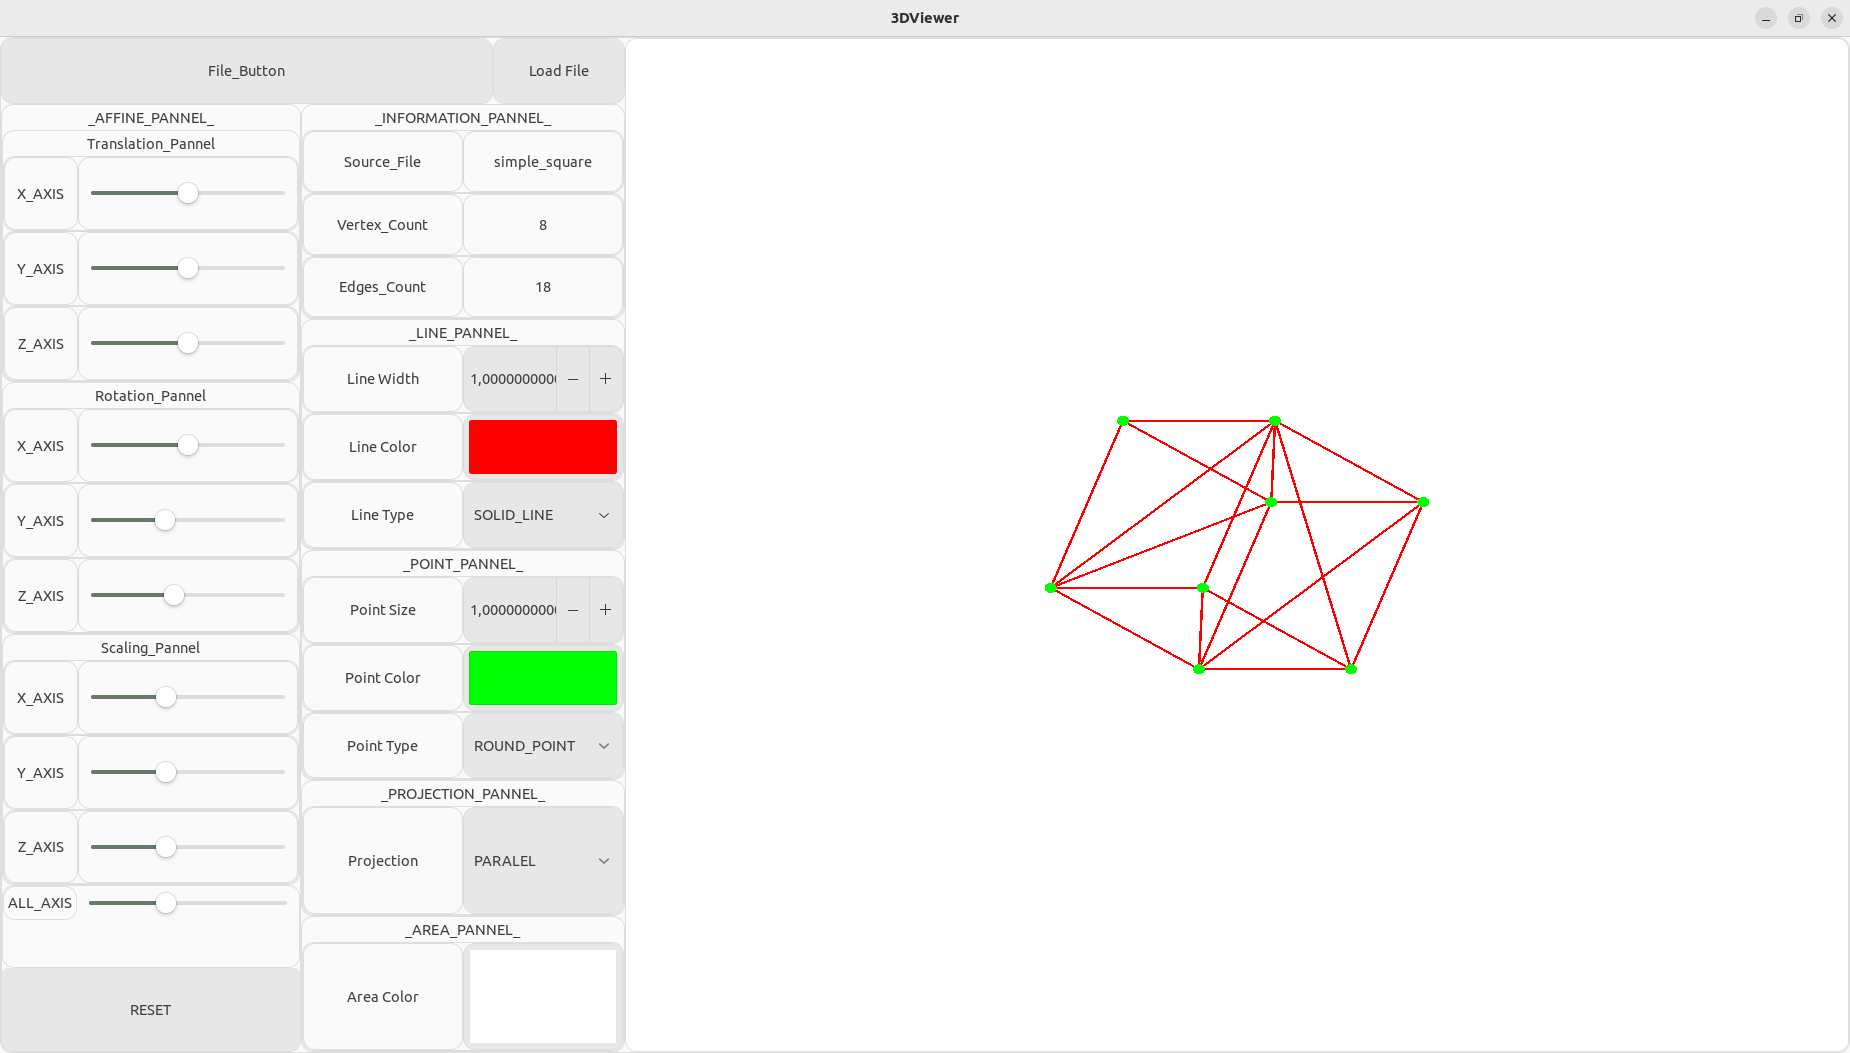
\includegraphics[width=1.3\textwidth]{2}
	\vspace*{\fill}
	\caption{Functional}
	\label{fig:func}
\end{figure}

\end{document}          
